\documentclass{beamer}


\mode<presentation>
{
  \usetheme{Darmstadt}
  \useoutertheme{infolines}
}

\usepackage{alltt}

\usepackage{etex}         % to avoid compilation erros of xypic
\usepackage[curve]{xypic}
%\xyoption{pdf}
%\usepackage[pdf]{xy}


\usepackage[utf8]{inputenc}
\usepackage{proof}
\inferLineSkip=4pt  % increase spacing between lines; default is 2pt

\usepackage{amsmath}
\usepackage{amssymb}
\usepackage{fontawesome}
\usepackage{times}
\usepackage[T1]{fontenc}
\usepackage{listings}
\lstset{language=haskell,basicstyle=\ttfamily}

\usepackage{multicol}
\usepackage{mathpartir}
\usepackage{mathtools}
\usepackage{stmaryrd}
\usepackage{soul}
\usepackage{tikzsymbols}

% Delete this, if you do not want the table of contents to pop up at
% the beginning of each subsection:
\AtBeginSection[]
{
  \begin{frame}<beamer>
    \frametitle{Plan}
    \tableofcontents[sectionstyle=show/shaded,subsectionstyle=hide]
  \end{frame}
}

\AtBeginSubsection[]
{
  \begin{frame}<beamer>
    \frametitle{Plan}
    \tableofcontents[sectionstyle=show/hide,subsectionstyle=show/shaded/hide]
%    \tableofcontents[subsectionstyle=show/shaded/hide]
  \end{frame}
}

\setbeamertemplate{footline}
{%
%\begin{beamercolorbox}{section in head/foot}
%\vskip2pt\insertnavigation{\paperwidth}\vskip2pt
%\end{beamercolorbox}%
\insertpagenumber
\insertshorttitle[width={5cm},center]
\insertshortinstitute[width={3cm},center]
\insertshortdate[width={3cm},center]
}


% If you wish to uncover everything in a step-wise fashion, uncomment
% the following command: 

%\beamerdefaultoverlayspecification{<+->}

\usepackage{tikz}
\usetikzlibrary{trees}
\usetikzlibrary{arrows}
\usetikzlibrary{decorations.pathmorphing}
\usetikzlibrary{shapes.multipart}
\usetikzlibrary{shapes.geometric}
\usetikzlibrary{calc}
\usetikzlibrary{positioning} 
\usetikzlibrary{fit}
\usetikzlibrary{backgrounds}
\usetikzlibrary{automata}


%%% Local Variables: 
%%% mode: latex
%%% TeX-master: "main"
%%% End: 

% Theorems and definitions

% \newtheorem{definition}{Definition}
% \newtheorem{theorem}{Theorem}
% \newtheorem{lemma}{Lemma}
% \newtheorem{proposition}{Proposition}


% Definition of colors
\newcommand{\blue}[1]{{\color{blue}#1}}
\newcommand{\green}[1]{{\color{green}#1}}
\newcommand{\red}[1]{{\color{red}#1}}
\newcommand{\gray}[1]{{\color{gray}#1}}

% From MSCS file
\newcommand{\eg}{\textit{e.g.\ }}
\newcommand{\etal}{\textit{et al.\ }}
\newcommand{\etc}{\textit{etc}}
\newcommand{\ie}{\textit{i.e.\ }}
\newcommand{\viz}{\textit{viz.\ }}
\newcommand{\wrt}{\textit{w.r.t.\ }}
\newcommand{\lex}{\langle}
\newcommand{\rex}{\rangle}

% Own abbreviations
\newcommand{\secref}[1]{Section~\ref{#1}}
\newcommand{\secrefs}[1]{Sections~\ref{#1}}
\newcommand{\figref}[1]{Figure~\ref{#1}}
\newcommand{\figrefs}[1]{Figures~\ref{#1}}
\newcommand{\pgref}[1]{page~\pageref{#1}}
\newcommand{\theoremref}[1]{Theorem~\ref{#1}}
\newcommand{\theoremrefs}[1]{Theorems~\ref{#1}}
\newcommand{\lemmaref}[1]{Lemma~\ref{#1}}
\newcommand{\exampleref}[1]{Example~\ref{#1}}
\newcommand{\defref}[1]{Definition~\ref{#1}}

\newcommand{\figline}{\rule{\textwidth}{0.5pt}}


% Logique

\newcommand{\IMPL}[0]{\longrightarrow}
\newcommand{\IMPLL}[0]{\Longrightarrow} % another implication, to make
                                % a difference with reduction relations
\newcommand{\AND}[0]{\land}
\newcommand{\OR}[0]{\lor}
\newcommand{\NOT}[0]{\lnot}
\newcommand{\FALSE}[0]{\perp}
\newcommand{\TRUE}[0]{\top}
\newcommand{\IFF}[0]{\leftrightarrow}
\newcommand{\BIGAND}[1]{\bigwedge_{#1}}
\newcommand{\BIGOR}[1]{\bigvee_{#1}}
\newcommand{\BIGANDC}[2]{\bigwedge_{#1|#2}} % bigand with constraint
\newcommand{\BIGORC}[2]{\bigvee_{#1|#2}}    % bigor with constraint

\newcommand{\exgeq}[1]{\exists^{{\geq #1}}}
\newcommand{\exeq}[1]{\exists^{{= #1}}}
\newcommand{\exle}[1]{\exists^{{< #1}}}

% Other

\newcommand{\smalltalcq}[0]{{\small small}-t{$\cal ALCQ$}}
\newcommand{\smalltalcqe}[0]{{\small small}-t{$\cal ALCQ$e}}
\newcommand{\trule}[0]{\xhookrightarrow}
\newcommand{\tableaurule}[1]{{\xhookrightarrow[]{#1}}}
\newcommand{\nodes}[1]{{\cal N}({#1})}
\newcommand{\trans}[1]{{\cal T}({#1})}
\newcommand{\transm}[1]{{\cal T'}({#1})}
\newcommand{\rconts}[1]{\llparenthesis #1 \rrparenthesis} %record contents
\newcommand{\rupd}[2]{{#1}\llparenthesis #2 \rrparenthesis} %record update

\newcommand{\eform}[0]{\mathit{eform}}
\newcommand{\form}[0]{\mathit{form}}
\newcommand{\free}[0]{\mathit{free}}
\newcommand{\exclprop}[0]{\stackrel{\times}{\longrightarrow}}


%----------------------------------------------------------------------
% For drawing syntax diagrams
% ----------------------------------------------------------------------

% Environment defining the general layout

\newenvironment{syntaxdiagram}[1]
{
%  \begin{equation}\label{eq:#1}
  \begin{tikzpicture}[%
node distance=5mm and 10mm,
>=stealth',
black!50,
text=black,
graphs/every graph/.style={edges=rounded corners},
hv path/.style={to path={-| (\tikztotarget)}},
vh path/.style={to path={|- (\tikztotarget)}},
nonterminal/.style={%
rectangle,
minimum size=6mm,
draw=black,
},
terminal/.style={%
rectangle,minimum size=6mm,rounded corners=3mm,
draw=black!50,
},
start/.style={%
circle,inner sep=1pt,minimum size=1pt,fill=white,draw=black!50,
},
end/.style={%
start,
},
junction/.style={circle,inner sep=0pt,minimum size=0pt},]
\node[nonterminal] (#1) {\hypertarget{syn:#1}{#1:}};
}
{\end{tikzpicture}
%\end{equation}
}

% Connects start point #1 via intermediate node entry #2 and exit #3
% to an end point #4.
\newcommand{\syndiagAlternative}[4]{%
\graph[use existing nodes] {
#1 ->[vh path] #2;
#3 ->[hv path] #4;
};
}

% Connects start point #1 via intermediate node #2 (typically a junction)
% to an end point #3.
\newcommand{\syndiagBridge}[3]{%
\graph[use existing nodes] {
#1 --[vh path] #2;
#2 ->[hv path] #3;
};
}

\newcommand{\nonterminalref}[1]{\hyperlink{syn:#1}{#1}}


%----------------------------------------------------------------------
% Remarks
% ----------------------------------------------------------------------

\newcommand{\remms}[2][]{\todo[color=green!40,#1]{MS: #2}}



%%% Local Variables: 
%%% mode: latex
%%% TeX-master: "main"
%%% End: 


\title{Timed Automata}

\author{Martin Strecker}
\date{2021-06-03}


%======================================================================

\begin{document}


%======================================================================

\begin{frame}
  \titlepage
\end{frame}



%======================================================================
\section{Timed Automata - Basic notions}



%-------------------------------------------------------------
\begin{frame}[fragile]\frametitle{Recap: Classical Finite-State Automata}
  
The chewing gum automaton:

  \begin{center}
    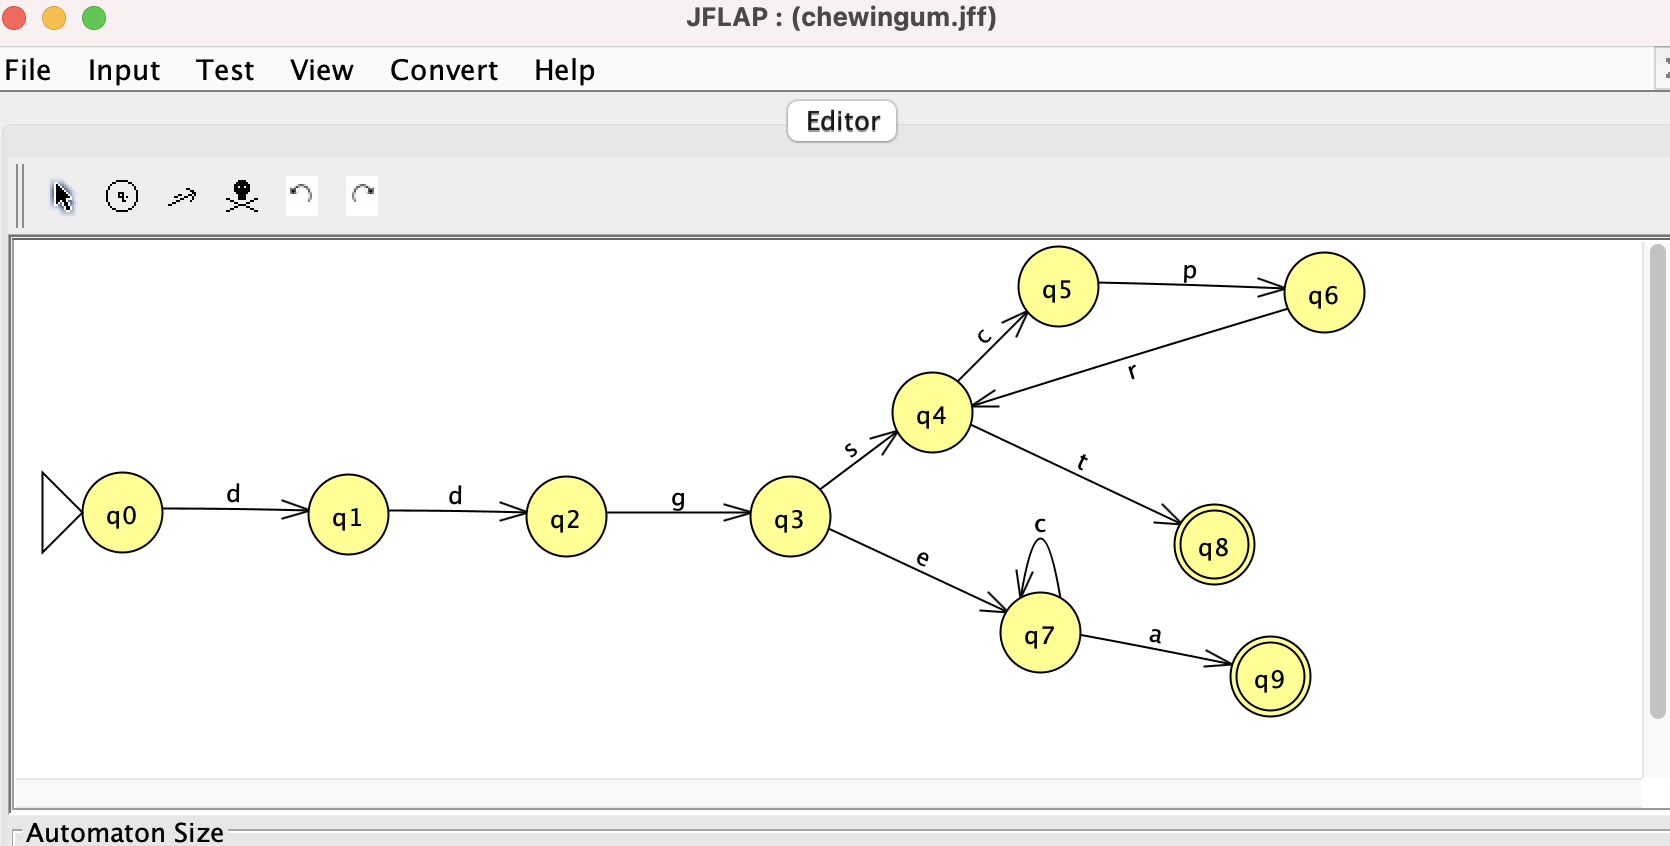
\includegraphics[scale=0.4]{Figures/chewing_gum_automaton.png}
  \end{center}

\end{frame}



%-------------------------------------------------------------
\begin{frame}[fragile]\frametitle{Recap: Classical Finite-State Automata}
  
  \blue{Central ingredients:}
  \begin{itemize}
  \item States (circles)
  \item Transitions (arcs between states) annotated with symbols of an alphabet
  \item One \emph{initial} state, marked with triangle (where execution starts)
  \item One or several \emph{final} states, marked by double circle (where execution ends)
  \end{itemize}


  \blue{Central notions:}
  \begin{itemize}
  \item Symbols of an alphabet represent possible \emph{actions}
  \item Accepted \emph{word} of an automaton: sequence of symbols leading from initial to final state
    \begin{itemize}
    \item \emph{Ex.:}  \texttt{ddgscprcprt} is accepted
    \item \emph{Ex.:} \texttt{dget} is not accepted
    \end{itemize}
    The set of accepted words of an automaton make up the \emph{language} recognized by the automaton. 
  \end{itemize}

\end{frame}


%-------------------------------------------------------------
\begin{frame}[fragile]\frametitle{Towards Timed Automata}

  \blue{What remains:} Notion of \emph{discrete state}\\
    not appropriate for \emph{continuous} actions (\emph{e.g.} ball rolling down a slope)

\vspace{5mm}
\blue{What is new:}
\begin{itemize}
\item Two kinds of transitions:
  \begin{itemize}
  \item \emph{Action} transition $\to^a$, inducing state change
  \item \emph{Delay} transition  $\to^d$, inducing progression of time
  \end{itemize}
\item Notion of timer / \emph{clock}
\item Further annotations on
  \begin{itemize}
  \item states (\emph{invariants})
  \item transitions (\emph{guards})
  \end{itemize}
\item Executions may be infinite
\end{itemize}

\end{frame}

%-------------------------------------------------------------
\begin{frame}[fragile]\frametitle{Using Uppaal}

  \begin{itemize}
  \item Download from \url{https://uppaal.org/downloads/}
  \item Unpack archive
  \item In the resulting repository:
    \begin{itemize}
    \item launch \texttt{./uppaal\&}
    \item \emph{or} run Java jar file: \texttt{java -jar uppaal.jar\&}
    \end{itemize}
  \item On Mac, it may be necessary to authorize file system access (?)
  \item Open project with \texttt{File / Open System}
  \end{itemize}

\end{frame}

%-------------------------------------------------------------
\begin{frame}[fragile]\frametitle{Some hints}

  \blue{File formats:}
  \begin{itemize}
  \item \texttt{*.xml} Full system information, incl.{} graphics and queries
  \item \texttt{*.xta} Human-readable textual format for automata, no graphics
    info, no queries
  \item \texttt{*.q} queries only
  \end{itemize}

  \blue{Edit node / transition info:}
  \begin{itemize}
  \item by double click on element
  \end{itemize}

  \blue{If information is scattered over the canvas:}
  \begin{itemize}
  \item Click on node / arc to see elements associated with it
  \end{itemize}

  \blue{Notable:}
  \begin{itemize}
  \item Initial state with double circle
  \item No final states (see: queries for verification)
  \end{itemize}
  
\end{frame}

%-------------------------------------------------------------
\begin{frame}[fragile]\frametitle{Example automaton}

  \begin{center}
    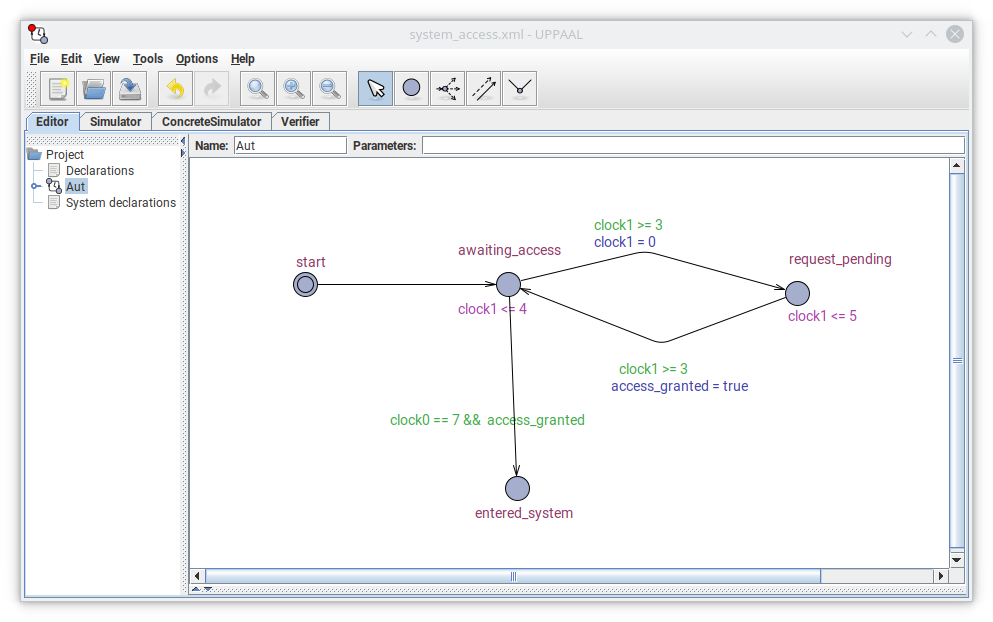
\includegraphics[scale=0.4]{Figures/system_access_automaton.png}
  \end{center}

  See: \texttt{fv} repository,  \texttt{Experiments/Uppaal/system\_access.xml}
\end{frame}

%-------------------------------------------------------------
\begin{frame}[fragile]\frametitle{Annotations}

  \blue{States} can be annotated with:
  \begin{itemize}
  \item \emph{invariant:} a condition to be satisfied to remain in this state.\\
    \emph{e.g.:} \texttt{clock1 <= 4} of \texttt{awaiting\_access}
  \end{itemize}

  \vspace{3mm}
  \blue{Transitions} can be annotated with:
  \begin{itemize}
  \item \emph{guard:} a condition to be satisfied to take the transition\\
        \emph{e.g.:} \texttt{clock1 >= 3} 
  \item \emph{update:} an assignment to a clock or data variable:
         \texttt{clock1 = 0} 
      \item \emph{synchronisation} of the form \texttt{e!} (send event) or
        \texttt{e?} (receive event)
  \end{itemize}

  \vspace{3mm}
  \emph{Note:} a \blue{condition} is a conjunction of
  \begin{itemize}
  \item clock comparisons: \texttt{clock1 >= 3}
  \item non-temporal Boolean conditions (\texttt{access\_granted})
  \end{itemize}
  
\end{frame}


%-------------------------------------------------------------
\begin{frame}[fragile]\frametitle{Traces}

  A \emph{configuration} consists of:
  \begin{itemize}
  \item a state 
  \item the values of the clocks
  \item the values of data variables
  \end{itemize}

  A \emph{trace} describes a sequence of transitions (action or delay) a TA can
  take. A trace is \emph{valid} if it respects the node and arc conditions.

  \vspace{3mm}
  For config (state, clock0, clock1, access\_granted):
  \begin{itemize}
  \item Example of valid trace:
  \[(start, 0, 0, false) \to^d (start, 2, 2, false) \to^a (aw, 2, 2, false) \to^d \]
  \[(aw, 3, 3, false) \to^a (req, 3, 0, false) \to^d (req, 7, 4, false) \to^a \]
  \[(aw, 7, 4, true) \to^a (entered, 7, 4, true) \]
  \item Example of invalid trace (arc constraint not satisfied):
  \[(start, 0, 0, false)  \to^a (aw, 0, 0, false) \to^a (entered, 0, 0, false)\]
  \end{itemize}
\end{frame}


%-------------------------------------------------------------
\begin{frame}[fragile]\frametitle{Using the simulator}
  
\end{frame}


%-------------------------------------------------------------
\begin{frame}[fragile]\frametitle{Verifying properties}

  Specify system properties with formulas of \blue{CTL} (Computation Tree Logic)

  \vspace{3mm}

  Two kinds of quantifiers:
  \begin{itemize}
  \item \blue{Path quantifiers} over alternative execution paths:
    \begin{itemize}
    \item $A \phi$: for all executions, $\phi$ holds
    \item $E \phi$: there exists an execution such that $\phi$
    \end{itemize}
  \item \blue{State quantifiers} over states on one path:
    \begin{itemize}
    \item $\Box \phi$ (ASCII: \texttt{[]}): for all states on the path, $\phi$ holds
    \item $\Diamond \phi$ (ASCII: \texttt{<>}): there exists a state on the path such that $\phi$
    \end{itemize}
  \end{itemize}
  
  \vspace{3mm}
  In Uppaal:
  \begin{itemize}
  \item \dots{} and in general in CTL:\\
    Quantifiers only come in pairs $A \Box, A \Diamond, E \Box, E \Diamond$
  \item Apart from that, quantifiers cannot be nested.
  \end{itemize}
  
\end{frame}


%-------------------------------------------------------------
\begin{frame}[fragile]\frametitle{Path and state quantifiers, graphically}

  \begin{center}
    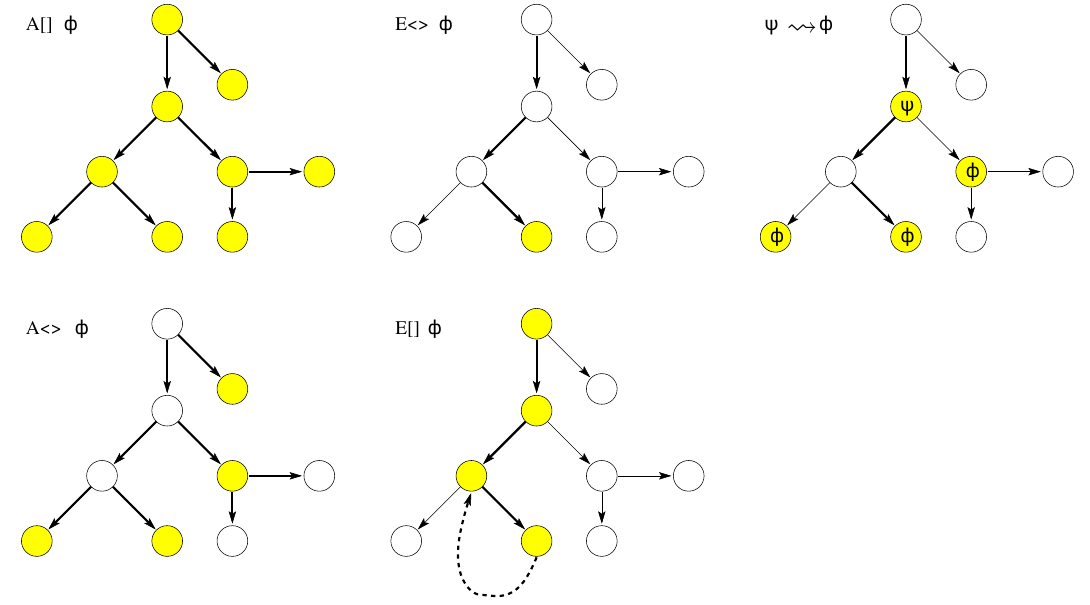
\includegraphics[scale=0.4]{Figures/path_and_state_quantifiers.png}
  \end{center}

\end{frame}


%-------------------------------------------------------------
\begin{frame}[fragile]\frametitle{Verifying properties in Uppaal}

  \begin{itemize}
  \item Open \texttt{Verifier} tab
  \item Type in formula (in \texttt{Query})
  \item Run \texttt{Check}, read off \texttt{Status}
  \item For:
    \begin{itemize}
    \item Satisfied existential properties
    \item Not satisfied universal properties
    \end{itemize}
    generate example / counterexample trace with \texttt{Get Trace}
  \item View trace in \texttt{Simulator} tab
  \end{itemize}

  \vspace{3mm}
  \emph{Example:} It is possible to enter the system:\\
  \texttt{E<> Aut.entered\_system}

  \vspace{3mm}
  \emph{Other queries} (possibly modify automaton):
  \begin{itemize}
  \item Sooner or later, one necessarily enters the system
  \item Clock1 always remains lower than 10
  \end{itemize}


\end{frame}





%======================================================================
\section{Timed Automata in Baby L4}


%-------------------------------------------------------------
\begin{frame}[fragile]\frametitle{Textual formats Uppaal / L4}

  \begin{itemize}
  \item Uppaal can be saved in human-readable \texttt{*.xta} format:
    \begin{itemize}
    \item \texttt{Save system as:} \texttt{system\_access.xta}
    \item save queries as \texttt{system\_access.q}
    \end{itemize}
  \item This is almost the L4 input format:
    \begin{itemize}
    \item Enclose system in declaration
    \item Change comments from \texttt{//} (Uppaal) to \texttt{\#} (L4)
    \item Move variable declarations to top level
    \item Rename some constants: \texttt{true} $\leadsto$ \texttt{True}
    \end{itemize}
  \end{itemize}
  
\end{frame}

%-------------------------------------------------------------
\begin{frame}[fragile]\frametitle{Textual format L4}

  \begin{lstlisting}
system Access {
bool access_granted;
process Aut() {
clock clock0, clock1;
state
    start,
    awaiting_access { clock1 <= 4 },
    request_pending { clock1 <= 5 },
    entered_system;
init
    start;
trans
    awaiting_access -> entered_system { guard clock0 == 7 ; },
    request_pending -> awaiting_access { guard clock1 >= 3;  },
    awaiting_access -> request_pending { guard clock1 >= 3; assign clock1 = 0; },
    start -> awaiting_access { }; } }

assert {printUp} True
  \end{lstlisting}
  

\end{frame}

%-------------------------------------------------------------
\begin{frame}[fragile]\frametitle{Work in Progress}

  \begin{itemize}
  \item TYpe checking of automata\\
    (needs generation of elements in the typing context: states, clocks,
    \dots)
  \item Structures and substructures (systems having automata as components)
  \item Model checking of complex systems via SMT 
  \item Difficulty: computation of fixed points
  \item Longer-reaching aim: Push the limits of what is currently possible in
    TA model checking (``parametric'' systems, more complex conditions)
  \end{itemize}

\end{frame}

%======================================================================
\section{Translating to Timed Automata}


%-------------------------------------------------------------
\begin{frame}[fragile]\frametitle{Approach~1: Actor-based}

  \begin{center}
    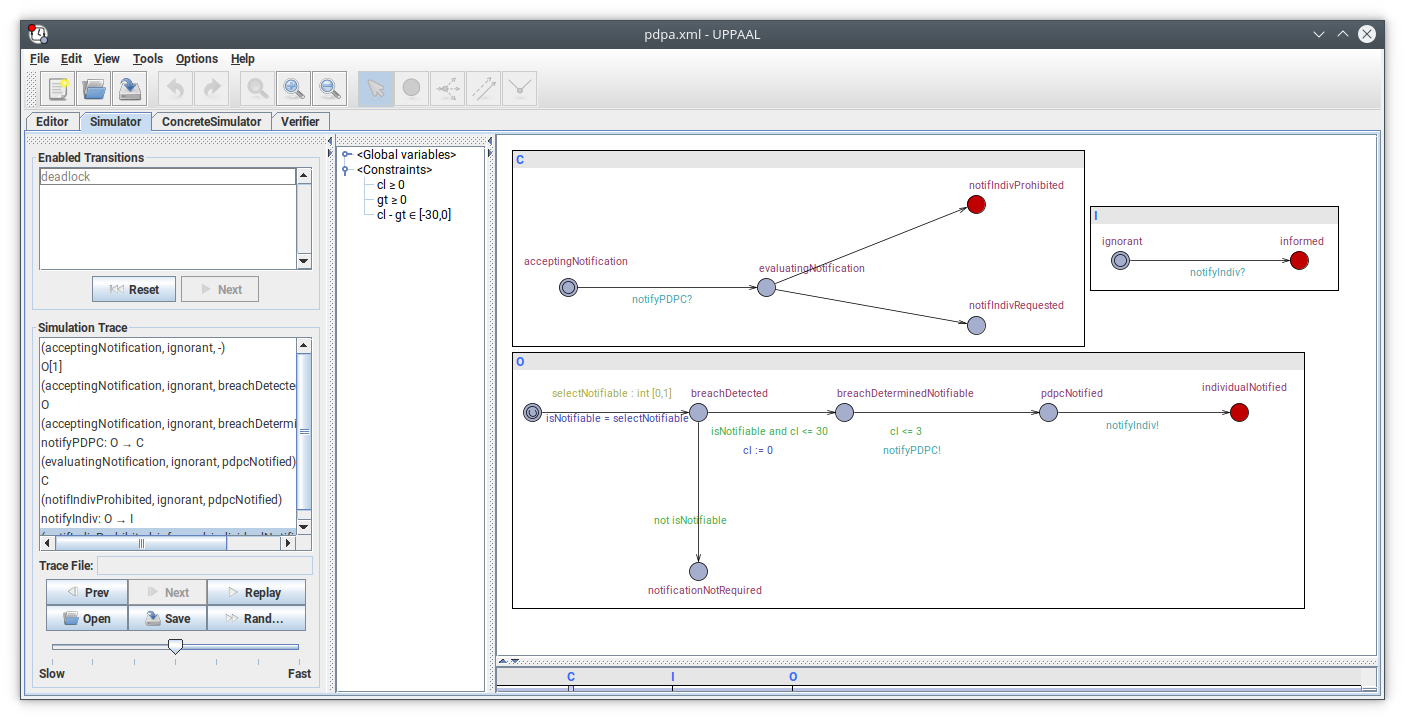
\includegraphics[scale=0.3]{Figures/actor_based_translation.png}
  \end{center}

\end{frame}


%-------------------------------------------------------------
\begin{frame}[fragile]\frametitle{Approach~2: Rule-based}

  \begin{center}
    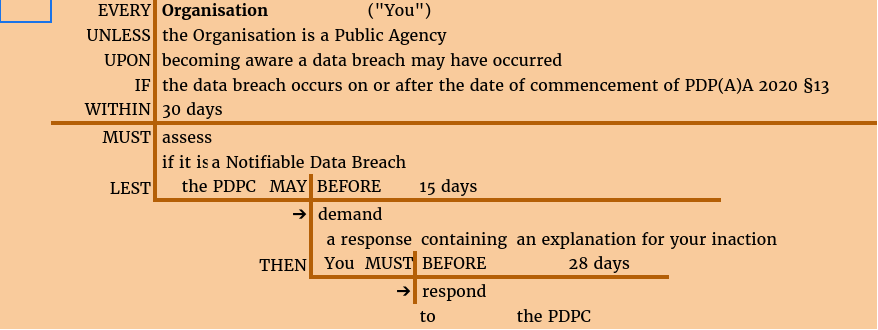
\includegraphics[scale=0.5]{Figures/rule_sf_l4.png}
  \end{center}

\end{frame}

%-------------------------------------------------------------
\begin{frame}[fragile]\frametitle{Approach~2: Rule-based}

  \begin{center}
    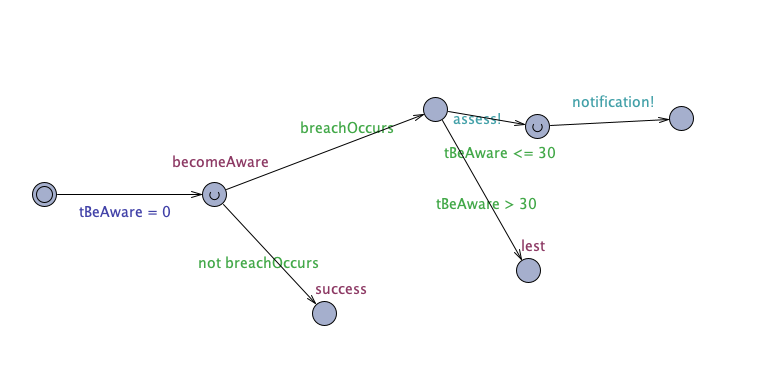
\includegraphics[scale=0.4]{Figures/rule_based_translation.png}
  \end{center}

\end{frame}


%-------------------------------------------------------------

\end{document}


%%% Local Variables: 
%%% mode: latex
%%% TeX-master: t
%%% coding: utf-8
%%% End: 
